\documentclass[cn]{elegantbook}
\usepackage[square,numbers,sort&compress]{natbib}
\newcommand{\upcite}[1]{\textsuperscript{\textsuperscript{\cite{#1}}}}
\usepackage{diagbox}
\usepackage{algorithm}
\usepackage{algorithmicx}
\usepackage{algpseudocode}
\usepackage{longtable}
\renewcommand{\algorithmicrequire}{\textbf{输入:}}
\renewcommand{\algorithmicensure}{\textbf{输出:}}

\tikzstyle{startstop} = [rectangle, rounded corners, minimum width = 2cm, minimum height=1cm,text centered, draw = black, fill = red!40]
\tikzstyle{arrow} = [->,>=stealth]

% title info
\title{模式识别大作业}
\subtitle{Caltech256图像分类}
% bio info
\author{罗雁天}
\institute{清华大学电子系}
\version{2018310742}
\date{\today}
\logo{logo.png}
\cover{cover.jpg}

\begin{document}

\maketitle
\tableofcontents
\mainmatter
\hypersetup{pageanchor=true}
% add preface chapter here if needed
\chapter{引言}
Caltech 256数据集是加利福尼亚理工学院收集整理的数据集,该数据集选自Google Image 数据集,并手工去除了不符合其类别的图片。在该数据集中,图片被分为256类,每个类别的图片超过80张。图\ref{intro}展示了Caltech 256数据集中其中20类图片的示例。

\begin{figure}[!h]
	\centering
	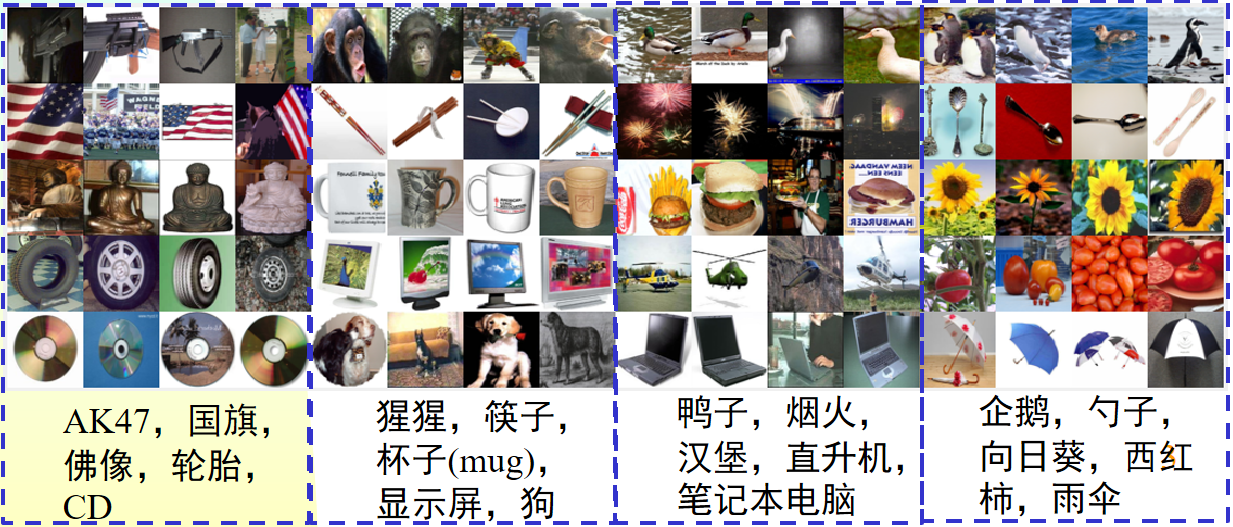
\includegraphics[width=\linewidth]{intro}
	\caption{\label{intro}Caltech 256数据集中其中20类图片示例}
\end{figure}

本次大作业在Caltech 256数据集的基础上复习和熟悉模式识别课上学习到的相关算法,完成如下几部分内容:
\begin{itemize}
	\item PCA/Fisher图像分类。采用PCA方法或Fisher线性判别准则进行特征变换,然后使用K近邻分类算法对选出的20类图片进行分类,分析选取不同主分量个数对识别率和虚警率的影响;并且进行开集测试;
	\item 使用其他特征和方法进行图像分类,比如HOG特征+SVM分类,同样进行开集测试,并比较以上两种方法的优缺点;
	\item (选做1)在全体257类图像上使用以上两种方法进行分类;
	\item (选做2)用深度学习的方法在原始数据集上进行图像分类;
\end{itemize}

\chapter{PCA降维+KNN分类}
\section{算法描述}
在本部分我们使用图像的像素值作为特征,使用PCA进行降维,然后再使用KNN进行分类。由于数据集中的图片大小不全相同,图像类型也不尽相同(有灰度图和彩色图),因此,在我们使用PCA降维之前需要首先对图像进行预处理,预处理的算法如Algorithm \ref{alg:preprocess}所示。

\begin{algorithm}[htb]
	\caption{图像预处理算法}
	\label{alg:preprocess}
	\begin{algorithmic}[1]
		\Require 原始图片$X$
		\Ensure 预处理之后的图片向量$X'$
		\State 首先将图片resize到统一大小$224\times 224$;
		\State 归一化处理$X = X / 255$,将像素值归一化到$[0,1]$区间内;
		\State 将单通道的灰度图通过复制通道变为3通道的图,彩色图不变;
		\State 最后将像素值拉平成一个向量,方便之后的PCA,$X'=X.flatten()$.
	\end{algorithmic}
\end{algorithm}

在图像预处理之后,由于我们处理之后的图像为$224\times224\times 3$,特征数量很多,直接使用KNN进行分类非常复杂并且耗时较多,并且在这么多的像素中有些像素肯定是对分类无关紧要的,因此,我们采用PCA算法首先对预处理之后的数据集进行降维,如Algorithm \ref{alg:pca}所示。

\begin{algorithm}[htb]
	\caption{图像PCA降维}
	\label{alg:pca}
	\begin{algorithmic}[1]
		\Require 预处理之后的训练集图片向量$X\in \mathbb{R}^{N\times50176}$,主成分数量$K$
		\Ensure PCA降维重建之后的$X'\in \mathbb{R}^{N\times k}$
		\State 将$X$进行中心化$X=X-mean(X, 1)$
		\State 计算$X$的协方差矩阵$\Sigma = X^TX$;
		\State 对$\Sigma$进行特征值分解;
		\State 将前$K$个最大特征值对应的特征向量组成投影矩阵$W$;
		\State 计算投影$y=W^T(X-\mu)$;
		\State  计算重建向量$x'=Wy+\mu$;
	\end{algorithmic}
\end{algorithm}

在PCA降维之后,我们使用KNN算法进行分类,如Algorithm \ref{alg:knn}所示。

\begin{algorithm}[htb]
	\caption{KNN分类}
	\label{alg:knn}
	\begin{algorithmic}[1]
		\Require 训练集($X,Y$),测试数据($z$)
		\Ensure 测试数据的类别
		\State 初始化k近邻的集合$knnlist$为前$k$个点,与k近邻距离的集合$distlist$为到前$k$个点的距离
		\For {$x\in X$}
		\State 计算距离最大的近邻为$maxk$,最大距离为$maxdist$
		\State 计算$x,z$之间的距离$dist$
		\If {$dist<maxdist$}
		\State 将$x$加入$knnlist$并将$maxk$在$knnlist$里删掉;
		\State 将$dist$加入$distlist$并将$maxdist$在$knnlist$里删掉;
		\EndIf
		\EndFor
		\State 统计$k$个最近邻样本中每个类别出现的次数
		\State 选择出现频率最大的类别作为未知样本的类别
	\end{algorithmic}
\end{algorithm}

\section{实验结果}
由于在此问题中,我们使用像素值作为特征,这样的话特征数量大于样本数量,所以我们设置主成分分量的时候要小于样本数量。在此,我们设置主成分分量为$1:5:1000$,观察对于不同的主成分分量的个数,识别率和虚警率的情况。在此,识别率和虚警率均指整体识别率和整体虚警率,计算方式如下:
\begin{equation}
\begin{aligned}
&P_{T P}=\frac{\sum_{i=1}^{c} N_{i, j}}{\sum_{i=1}^{c} N_{i}}\\
&P_{F P}=\frac{\sum_{i=1, \ldots, c, j=1, \ldots, c, i \neq j} N_{i, j}}{(c-1) * \sum_{j=1, \ldots, c} N_{j}}
\end{aligned}
\end{equation}

\subsection{在KNN算法中取$k=1$时}
绘制出识别率和虚警率随主成分个数的变化曲线如图\ref{knn_res_1}所示,从图中可以看出,随着主成分数量的增加,最开始识别率呈现递增趋势,在达到最高点之后,识别率有所下降并趋于稳定,这可能就是因为我们的特征数量高于样本数量的原因吧,并且直接使用像素作为特征可能分类效果也不好。从中我们可以看出,当主成分数量为51左右时,识别率较高,此时的识别率为0.2928709055876686,虚警率为0.03721732075854376。我们绘制出此时的混淆矩阵如图\ref{cm_1}所示。

\begin{figure}[!h]
	\centering
	\begin{minipage}[t]{0.48\textwidth}
		\centering
		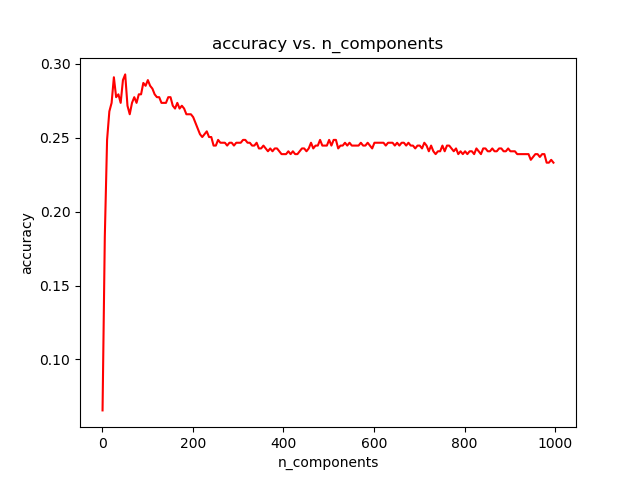
\includegraphics[width=\textwidth]{../results/acc_n_1}
	\end{minipage}
	\begin{minipage}[t]{0.48\textwidth}
		\centering
		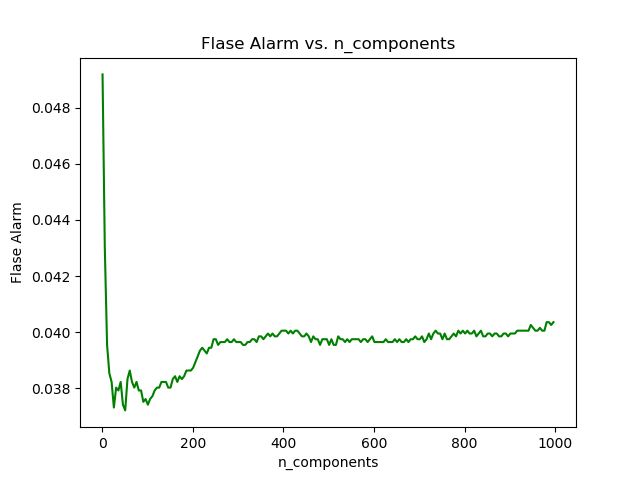
\includegraphics[width=\textwidth]{../results/falseAlarm_n_1}
	\end{minipage}
	\caption{\label{knn_res_1}$k=1$时结果图。左图:识别率变化曲线;右图:虚警率变化曲线}
\end{figure}

\begin{figure}[!h]
	\centering
	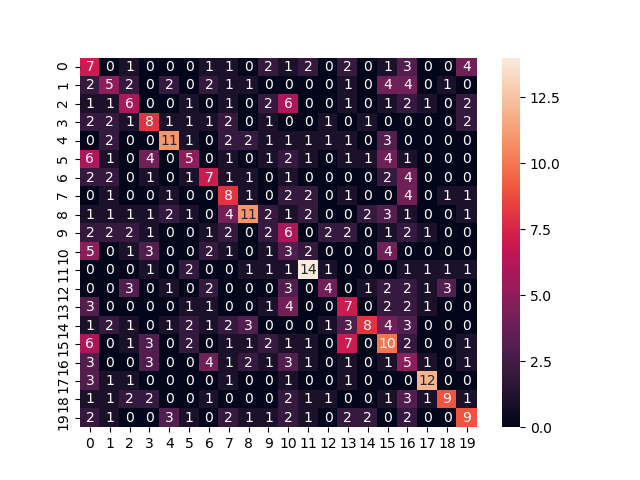
\includegraphics[width=0.9\linewidth]{../results/cm_1}
	\caption{\label{cm_1}$k=1, n\_components=51$时混淆矩阵图}
\end{figure}

\subsection{在KNN算法中取$k=3$时}
绘制出识别率和虚警率随主成分个数的变化曲线如图\ref{knn_res_2}所示,从中我们可以看出,当主成分数量为31左右时,识别率较高,此时的识别率为0.28901734104046245,虚警率为0.03742013994523882。我们绘制出此时的混淆矩阵如图\ref{cm_2}所示。

\begin{figure}[!h]
	\centering
	\begin{minipage}[t]{0.48\textwidth}
		\centering
		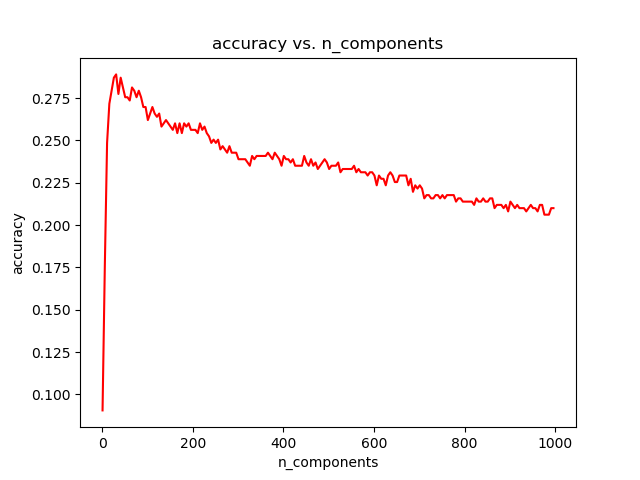
\includegraphics[width=\textwidth]{../results/acc_n_3}
	\end{minipage}
	\begin{minipage}[t]{0.48\textwidth}
		\centering
		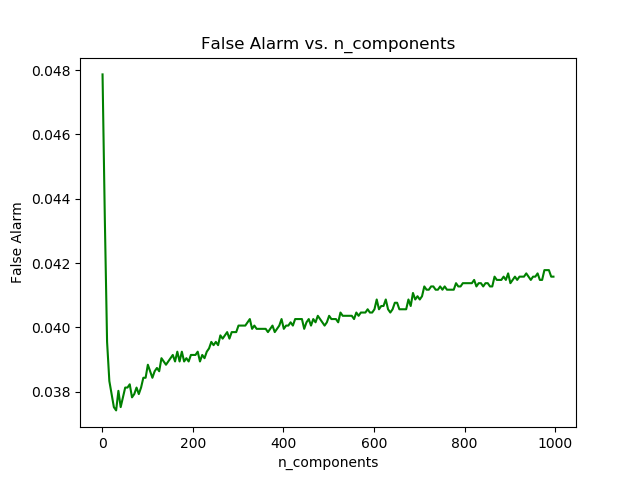
\includegraphics[width=\textwidth]{../results/falseAlarm_n_3}
	\end{minipage}
	\caption{\label{knn_res_2}$k=3$时结果图。左图:识别率变化曲线;右图:虚警率变化曲线}
\end{figure}

\begin{figure}[!h]
	\centering
	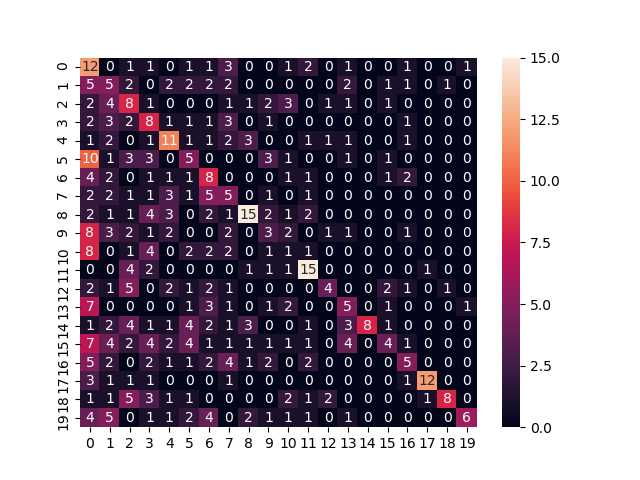
\includegraphics[width=0.9\linewidth]{../results/cm_3}
	\caption{\label{cm_2}$k=3, n\_components=31$时混淆矩阵图}
\end{figure}

\subsection{在KNN算法中取$k=5$时}
绘制出识别率和虚警率随主成分个数的变化曲线如图\ref{knn_res_3}所示,从中我们可以看出,当主成分数量为21左右时,识别率较高,此时的识别率为0.31021194605009633,虚警率为0.036304634418415985。我们绘制出此时的混淆矩阵如图\ref{cm_3}所示。

\begin{figure}[!h]
	\centering
	\begin{minipage}[t]{0.48\textwidth}
		\centering
		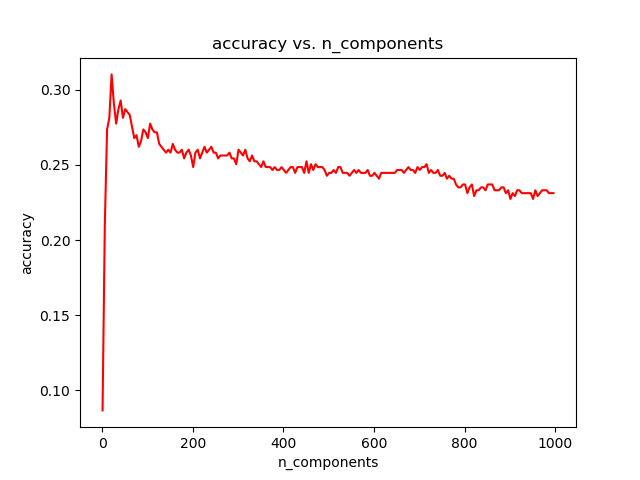
\includegraphics[width=\textwidth]{../results/acc_n_5}
	\end{minipage}
	\begin{minipage}[t]{0.48\textwidth}
		\centering
		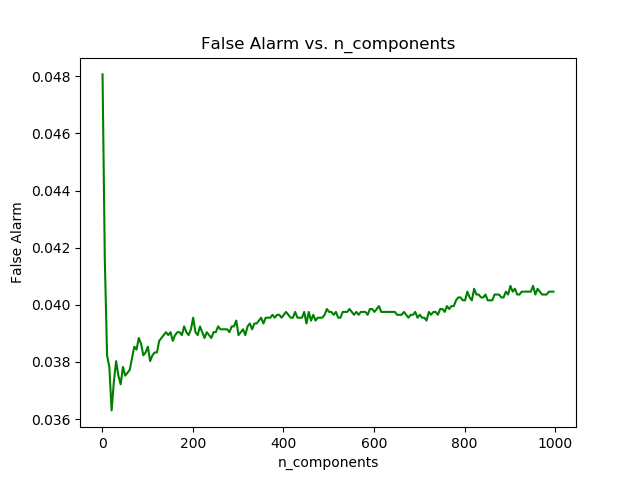
\includegraphics[width=\textwidth]{../results/falseAlarm_n_5}
	\end{minipage}
	\caption{\label{knn_res_3}$k=5$时结果图。左图:识别率变化曲线;右图:虚警率变化曲线}
\end{figure}

\begin{figure}[!h]
	\centering
	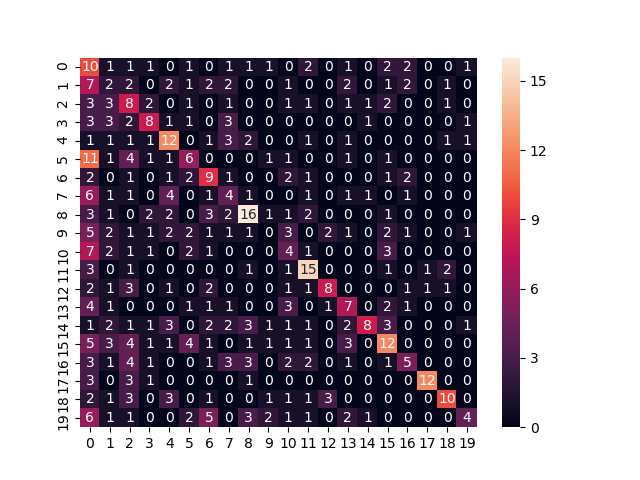
\includegraphics[width=0.9\linewidth]{../results/cm_5}
	\caption{\label{cm_3}$k=5, n\_components=21$时混淆矩阵图}
\end{figure}

\section{开集测试}
在此部分,我们不仅需要分类20类物体,还要对背景进行拒识,为此,我们选择Caltech 256数据集中第257类背景类中不在提供的test\_neg.txt中的部分图片进行训练,使用的图片保存在train\_neg.txt中。将其转换为一个21分类的问题。由于在之前的部分已经讨论过了实验结果与KNN中的k、PCA中主成分数量之间的关系,因此在本部分开集测试不再对此进行对比实验,我们选择$k=1, n\_components=[1:5:500]$进行实验,绘制出识别率和虚警率随主成分个数的变化曲线如图\ref{knn_res_1_open}所示,从中我们可以看出,当主成分数量为126左右时,识别率较高,此时的识别率为0.30737134909596664,虚警率为0.03674694385476905,我们绘制出此时的混淆矩阵如图\ref{cm_1_open}所示。

\begin{figure}[!h]
	\centering
	\begin{minipage}[t]{0.48\textwidth}
		\centering
		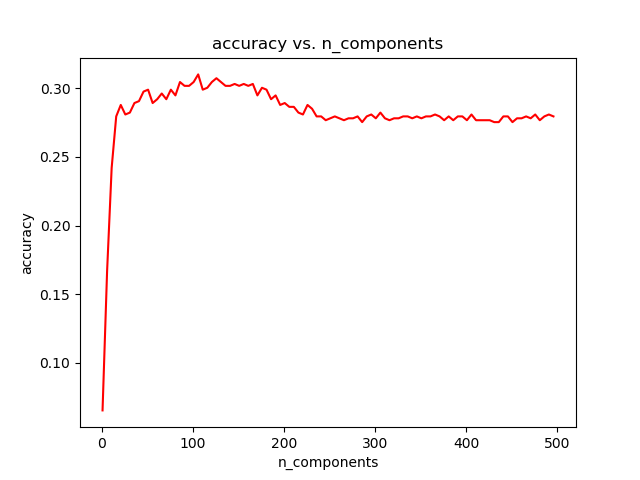
\includegraphics[width=\textwidth]{../results/acc_n_1_open}
	\end{minipage}
	\begin{minipage}[t]{0.48\textwidth}
		\centering
		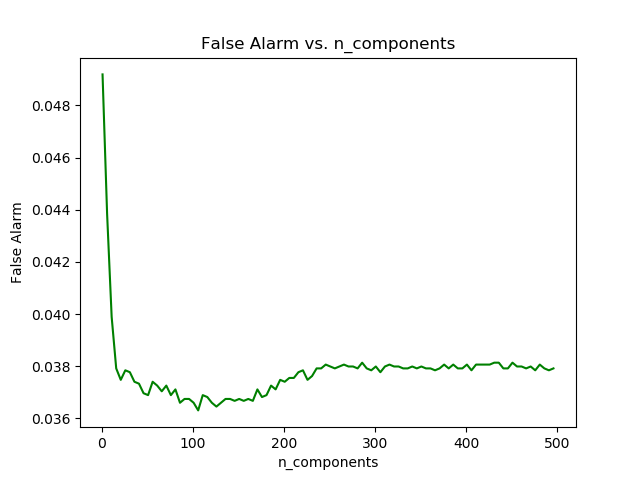
\includegraphics[width=\textwidth]{../results/falseAlarm_n_1_open}
	\end{minipage}
	\caption{\label{knn_res_1_open}$k=1$时结果图。左图:识别率变化曲线;右图:虚警率变化曲线}
\end{figure}

\begin{figure}[!h]
	\centering
	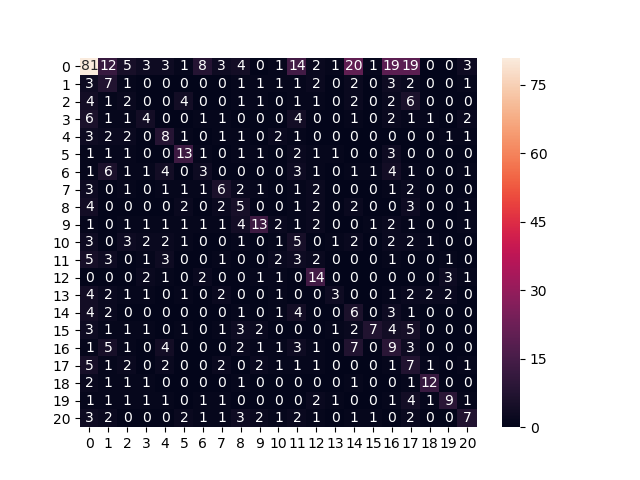
\includegraphics[width=0.9\linewidth]{../results/cm_1_open}
	\caption{\label{cm_1_open}$k=1, n\_components=126$时混淆矩阵图}
\end{figure}
\chapter{HoG特征+SVM分类}
\section{算法描述}
在上一章,我们使用像素值作为特征直接进行分类,可以看出,分类的正确率略低,在本章,我们使用HoG算法提取图片的HOG特征,然后使用SVM算法进行多分类。

方向梯度直方图(Histogram of Oriented Gradient, HOG)特征是一种在计算机视觉和图像处理中用来进行物体检测的特征描述子。它通过计算和统计图像局部区域的梯度方向直方图来构成特征。Hog特征结合SVM分类器已经被广泛应用于图像识别中,尤其在行人检测中获得了极大的成功。因此在此问题上,我们也才用此种分类方法来尝试进行分类。

使用HoG算法提取特征之后我们使用SVM算法进行分类,SVM算法主要是针对二分类问题,对于我们的问题主要有两种思路:训练每一类和其他所有类的分类界面(ovr),训练每两类之间的分类界面(ovo),在本实验中,我们选择了ovr的方式进行多分类。

\section{实验结果}
通过多次尝试,在使用线性核SVM时HoG特征提取算法的最优参数及识别率、虚警率如表\ref{hog_res1}所示,对应的混淆矩阵如图\ref{hog_svm_lin}所示。从实验结果来看,使用HoG特征提取算法能够提取一些较高级的特征,相比于直接用像素值作为特征来说要好很多,并且使用SVM分类能够针对线性可分、线性不可分问题有较好的分类界面,因此使用HoG特征+SVM分类的方式解决此问题要比PCA+KNN的方式得到的识别率要高,虚警率更低。但是使用HoG特征之后使用SVM不能根据自己的需求选择特征,并且HoG的特征数量较多,不适合于直接分类,所以可以将这两种算法进行结合,使用HoG+PCA+SVM的方式来解决此问题。如图\ref{hog_pca_svm_lin}是使用HoG+PCA+SVM的方式分类的混淆矩阵示意图,在选择主成分数量为700的条件下,最优的识别率为45.87\%,虚警率为0.02849,可以看出,在使用PCA之后识别率有略微提升,并且特征数量相比于直接使用HoG有明显减少。
\begin{table}[!h]
	\centering
	\caption{\label{hog_res1}HoG+线性SVM最优参数及其对应的识别率、虚警率}
	\begin{tabular}{|c|c|c|c|c|c|}
		\hline
		orientations & block\_norm & pixels\_per\_cell & cells\_per\_block & 识别率 & 虚警率 \\
		\hline
		13 & L1 & [8,8] & [4,4] & 45.66\% & 0.028597 \\
		\hline
	\end{tabular}
\end{table}

\begin{figure}[!h]
	\centering
	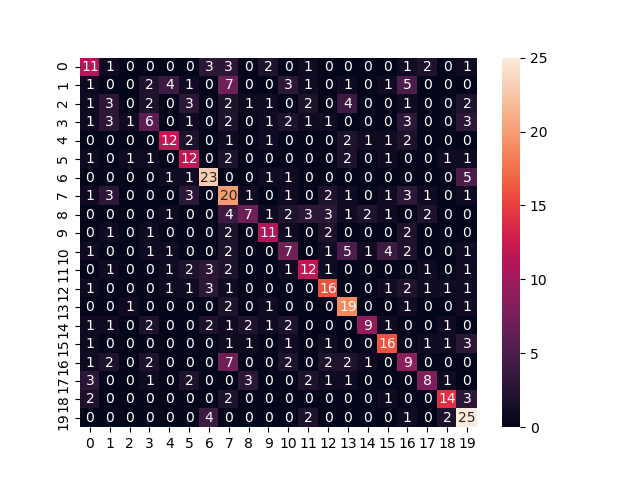
\includegraphics[width=\linewidth]{../results/hog_svm_lin}
	\caption{\label{hog_svm_lin}HoG+线性SVM分类时混淆矩阵图}
\end{figure}

\begin{figure}[!h]
	\centering
	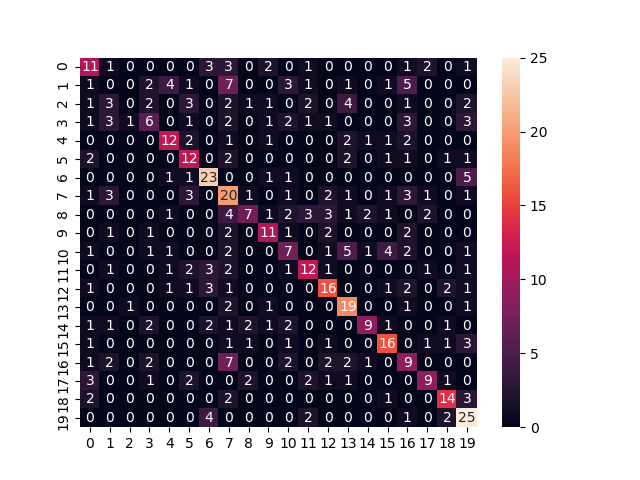
\includegraphics[width=\linewidth]{../results/hog_pca_svm_lin}
	\caption{\label{hog_pca_svm_lin}HoG+PCA+线性SVM分类时混淆矩阵图}
\end{figure}

\section{开集测试}
与上一章节开集测试类似,我们依然选择Caltech 256数据集中第257类背景类中不在提供的test\_neg.txt中的部分图片进行训练,使用的图片保存在train\_neg.txt中。同样的,我们使用HoG+SVM和HoG+PCA+SVM两种方式对此进行分类,实验结果如表\ref{hog_res2}所示,相对应的混淆矩阵如图\ref{hog_svm_lin_open}和\ref{hog_pca_svm_lin_open}所示,可以看出使用PCA降维之后的效果还是相比于直接进行SVM的效果好。

\begin{table}[!h]
	\centering
	\caption{\label{hog_res2}开集测试时的识别率、虚警率}
	\begin{tabular}{|c|c|c|}
		\hline
		分类方法 & 识别率 & 虚警率 \\
		\hline
		HoG+SVM & 47.42698\% & 0.02767 \\
		\hline
		HoG+PCA(n\_components=700)+SVM & 47.70515\% & 0.02752 \\
		\hline
	\end{tabular}
\end{table}

\begin{figure}[!h]
	\centering
	\begin{minipage}{0.48\linewidth}
		\centering
		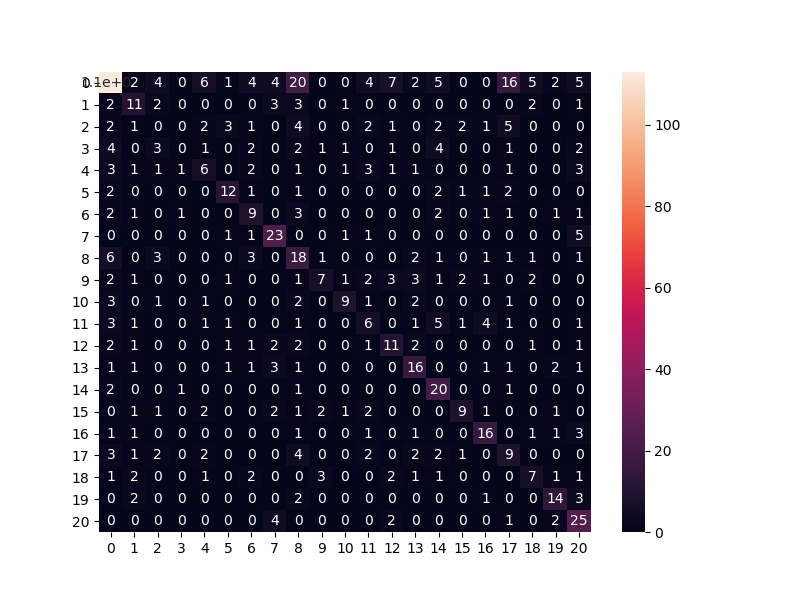
\includegraphics[width=\linewidth]{../results/hog_svm_lin_open}
		\caption{\label{hog_svm_lin_open}HoG+线性SVM分类开集测试时混淆矩阵图}
	\end{minipage}
	\begin{minipage}{0.48\linewidth}
		\centering
		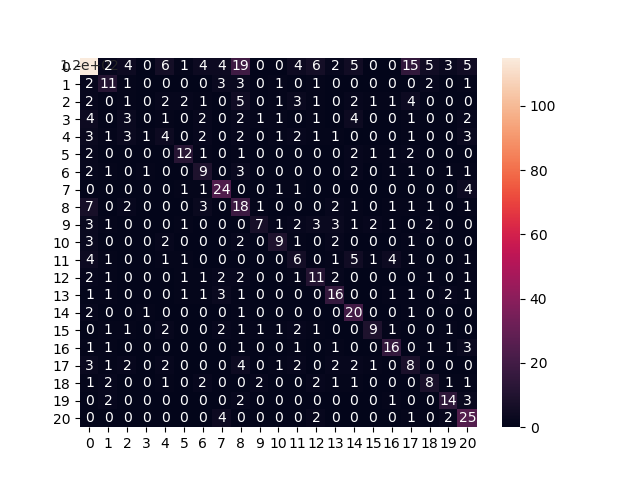
\includegraphics[width=\linewidth]{../results/hog_pca_svm_lin_open}
		\caption{\label{hog_pca_svm_lin_open}HoG+PCA+线性SVM分类开集测试时混淆矩阵图}
	\end{minipage}
\end{figure}

\chapter{(选做1)在全体257类图像上使用以上两种方法进行分类}
\section{训练集和测试集创建}
首先我们创建训练集和测试集,在此,我们在每一类样本中选择25张图片加入测试集,其余图片加入训练集中进行训练,由于使用的算法与之前两章提到的算法类似,在此不再赘述,并且,由于在全体数据集中已经加入了负样本,因此,在此部分也无需进行开集测试。

\section{PCA+KNN实验结果}
由于在之前章节已经对比了不同k和n\_components对实验结果的影响,因此(其实还有一方面的原因是电脑太破跑的太慢了emmm),本部分只使用k=5,n\_components=500来进行分类,最终的识别率为accuracy=8.7345\%,虚警率为0.048034。相比于随机分类的正确率1/257要高,但是我们也可以看出,使用此种方法在全体数据集上的分类效果还是很差的。分类后的混淆矩阵图如图\ref{cm_all}所示。

\begin{figure}[!h]
	\centering
	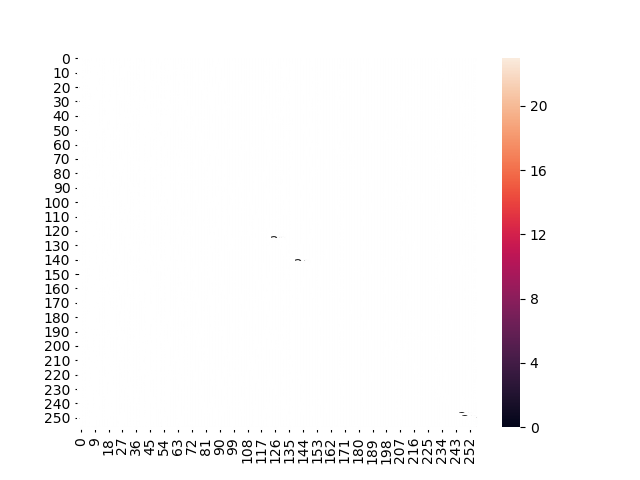
\includegraphics[width=0.9\linewidth]{../results/cm_pca_knn}
	\caption{\label{cm_all}$k=5, n\_components=500$时全体数据集混淆矩阵图}
\end{figure}
\section{HOG+SVM实验结果}
使用HoG+SVM算法得到的识别率为16.1045\%,虚警率为0.04415。相比于PCA+KNN效果稍微好点,但是识别率依然很低,与我们下一章节即将提到的神经网络分类的方法效果差很多。分类后的混淆矩阵图如图\ref{cm_all_1}所示。

\begin{figure}[!h]
	\centering
	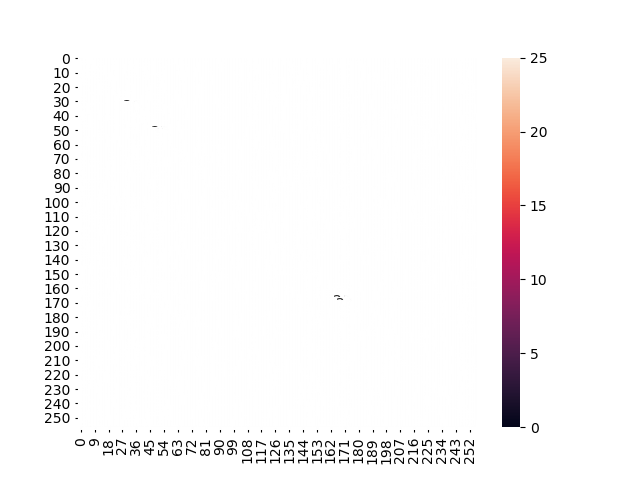
\includegraphics[width=0.9\linewidth]{../results/hog_svm_lin_all}
	\caption{\label{cm_all_1}HoG+SVM时全体数据集混淆矩阵图}
\end{figure}

\chapter{(选做2)在全体257类图像上使用CNN进行分类}
在本章,我们使用深度学习的方法对全体257类图像进行分类,首先我们创建训练集和测试集,在此,我们在每一类样本中选择25张图片加入测试集,其余图片加入训练集中进行训练。

\section{算法描述}
在本部分,我们使用ResNet和DenseNet网络结构进行实验,并且将实验结果进行对比。ResNet是由微软研究院的Kaiming He等四名华人提出,并且获得了ILSVRC2015的冠军,其核心结构为ResNet block(图\ref{resblock}),传统的卷积网络或者全连接网络在信息传递的时候或多或少会存在信息丢失,损耗等问题,同时还有导致梯度消失或者梯度爆炸,导致很深的网络无法训练。通过引入ResNet Block,避免了在反向传播中的梯度消失现象,能够设计很深的网络结构。
\begin{figure}[!h]
	\centering
	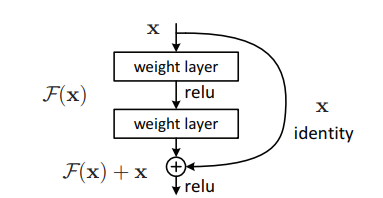
\includegraphics[width=\linewidth]{resblock}
	\caption{\label{resblock}ResNet Block示意图}
\end{figure}

DenseNet是2017年CVPR的Best Paper中提出来的网络结构,其脱离了加深网络层数(ResNet)和加宽网络结构(Inception)来提升网络性能的定式思维,从特征的角度考虑,通过特征重用和旁路(Bypass)设置,既大幅度减少了网络的参数量,又在一定程度上缓解了梯度消失问题的产生,其主要结构为密集连接模块(Dense Block),如图\ref{denseblock}所示。
\begin{figure}[!h]
	\centering
	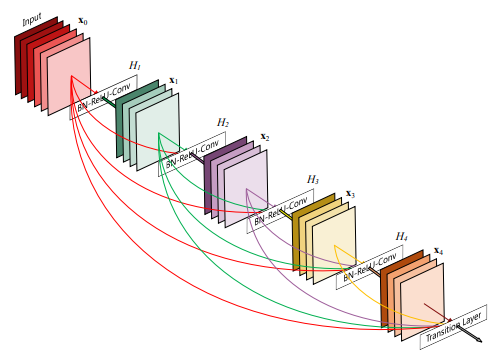
\includegraphics[width=0.9\linewidth]{denseblock}
	\caption{\label{denseblock}Dense Block示意图}
\end{figure}

\section{实验结果}
在本次实验中,我们尝试了多种网络结构与优化方法,使用ImageNet上预训练的参数进行训练,学习率采用步长衰减的方式设置,初始学习率为0.001.总体实验结果如表\ref{tab:res}所示:
\begin{table}[!h]
	\centering
	\caption{\label{tab:res}使用CNN进行分类的实验结果}
	\begin{tabular}{|c|c|c|c|c|}
		\hline
		网络结构 & 优化方法 & 损失函数 & test loss & test accuracy \\
		\hline
		DenseNet121 & SGD(finetune) & cross\_entropy & 83.48\% & 0.0427 \\
		\hline
		DenseNet121 & Adam(no finetune) & cross\_entropy & 78.26\% & 0.0140 \\
		\hline
		DenseNet121 & Adam(finetune) & cross\_entropy & {\color{red} 85.56\%} & {\color{red} 0.0087} \\
		\hline
		ResNet18 & Adam(finetune) & cross\_entropy & 80.36\% & 0.0119\\
		\hline
		ResNet18 & SGD(finetune) & cross\_entropy & 71.45\% & 0.0237\\
		\hline
	\end{tabular}
\end{table}

并且针对不同情况,我们都绘制出了train loss, train accuracy, test loss和test accuracy曲线进行对比。DenseNet121+SGD的曲线如图\ref{trainres_den}和\ref{testres_den}所示,在此次实验中,我们固定了除最后一层外的所有参数,均使用预训练的参数,而只通过训练微调最后一层的参数,因此可以看出收敛较快;

相比较而言,我们的第二次尝试,DenseNet121+Adam,我们虽然依然使用了预训练的参数,但是并没有固定除最后一层之外的其它层的参数,因此所有层的参数都是可以微调的,可以看出,此时的收敛速度并没有上一种情况的快,如图\ref{trainres_den_adam}和\ref{testres_den_adam}所示,从实验结果中可以看出,训练集的正确率明显高于测试集的正确率,这有可能是因为我们微调所有的参数使得可变化的参数量很多,有过拟合现象,因此在此问题中,我们固定其中一些参数可能能取得较好的效果。固定参数使用DenseNet121+Adam的实验结果如图\ref{trainres_den_adam1}和\ref{testres_den_adam1}所示,可以看出使用finetune方式的正确率更优,且收敛速度更快。

我们还使用了ResNet18作为网络结构对此问题进行分类,根据我们上面的讨论,在此我们还是使用finetune的方式进行训练,即固定除最后一层之外的其它层的参数,使用Adam优化算法的实验结果如图\ref{trainres_res_adam}和\ref{testres_res_adam}所示,使用SGD优化算法的实验结果如图\ref{trainres_res_sgd}和\ref{testres_res_sgd}所示,从实验结果中可以看出使用Adam优化算法进行实验比使用SGD优化算法的正确率和loss都要更优,并且我们还可以看出,使用Adam优化算法收敛速度也要比SGD快,这与我们之前在DenseNet121模型上对比的结果是一致的。
\begin{figure}[!h]
	\centering
	\begin{minipage}[t]{0.48\textwidth}
		\centering
		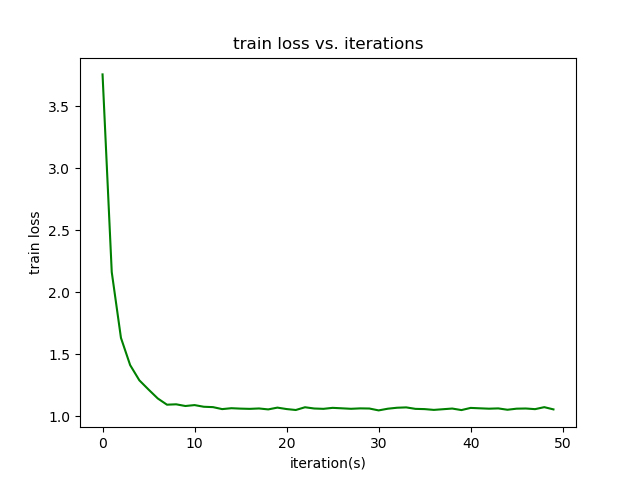
\includegraphics[width=\textwidth]{../results/trainloss_den}
	\end{minipage}
	\begin{minipage}[t]{0.48\textwidth}
		\centering
		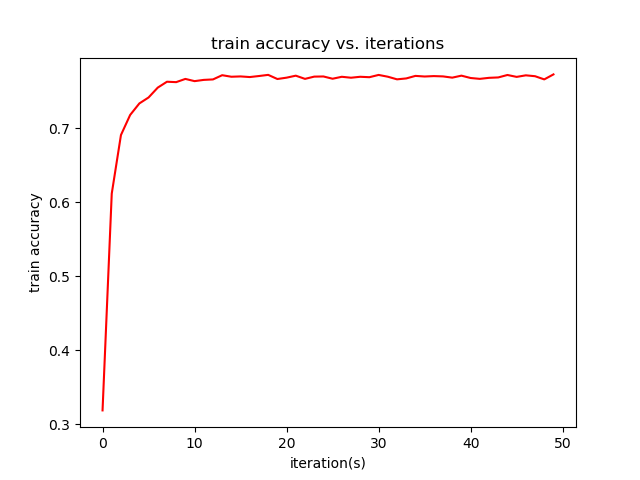
\includegraphics[width=\textwidth]{../results/trainacc_den}
	\end{minipage}
	\caption{\label{trainres_den}train loss curve and train accuracy curve using DenseNet121+SGD}
\end{figure}

\begin{figure}[!h]
	\centering
	\begin{minipage}[t]{0.48\textwidth}
		\centering
		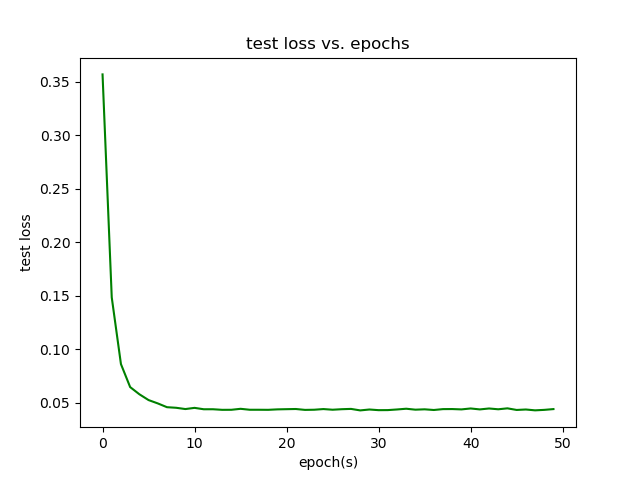
\includegraphics[width=\textwidth]{../results/testloss_den}
	\end{minipage}
	\begin{minipage}[t]{0.48\textwidth}
		\centering
		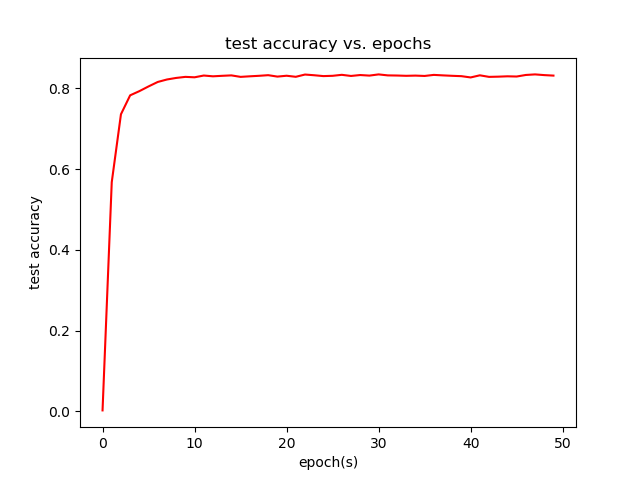
\includegraphics[width=\textwidth]{../results/testacc_den}
	\end{minipage}
	\caption{\label{testres_den}test loss curve and test accuracy curve using DenseNet121+SGD}
\end{figure}

\begin{figure}[!h]
	\centering
	\begin{minipage}[t]{0.48\textwidth}
		\centering
		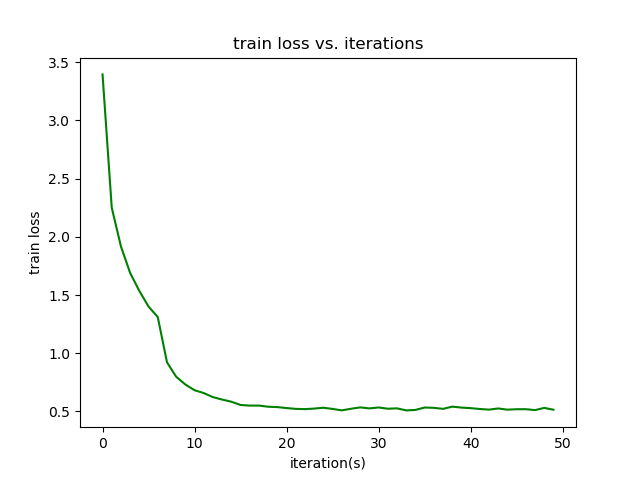
\includegraphics[width=\textwidth]{../results/trainloss_den_adam}
	\end{minipage}
	\begin{minipage}[t]{0.48\textwidth}
		\centering
		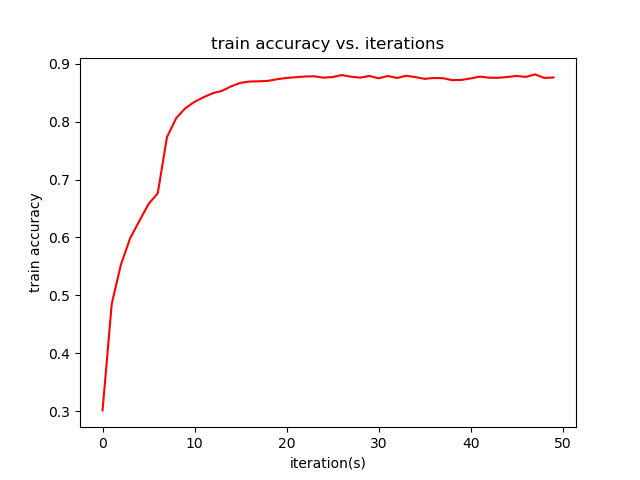
\includegraphics[width=\textwidth]{../results/trainacc_den_adam}
	\end{minipage}
	\caption{\label{trainres_den_adam}train loss curve and train accuracy curve using DenseNet121+Adam (without finetuning)}
\end{figure}

\begin{figure}[!h]
	\centering
	\begin{minipage}[t]{0.48\textwidth}
		\centering
		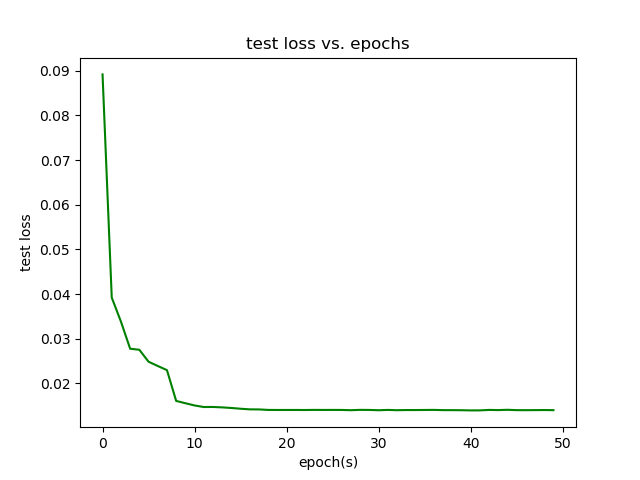
\includegraphics[width=\textwidth]{../results/testloss_den_adam}
	\end{minipage}
	\begin{minipage}[t]{0.48\textwidth}
		\centering
		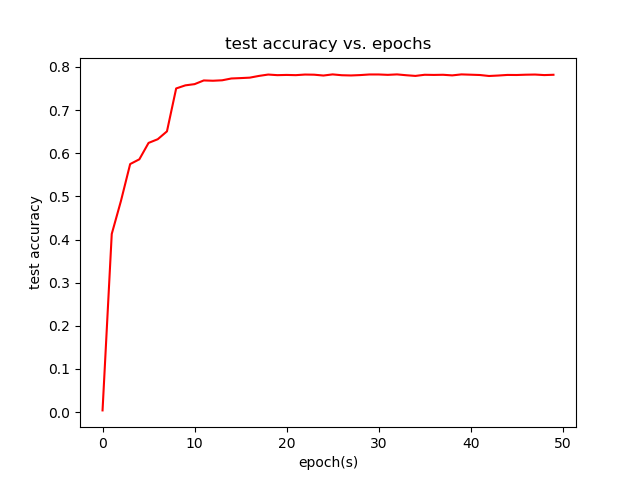
\includegraphics[width=\textwidth]{../results/testacc_den_adam}
	\end{minipage}
	\caption{\label{testres_den_adam}test loss curve and test accuracy curve using DenseNet121+Adam (without finetuning)}
\end{figure}

\begin{figure}[!h]
	\centering
	\begin{minipage}[t]{0.48\textwidth}
		\centering
		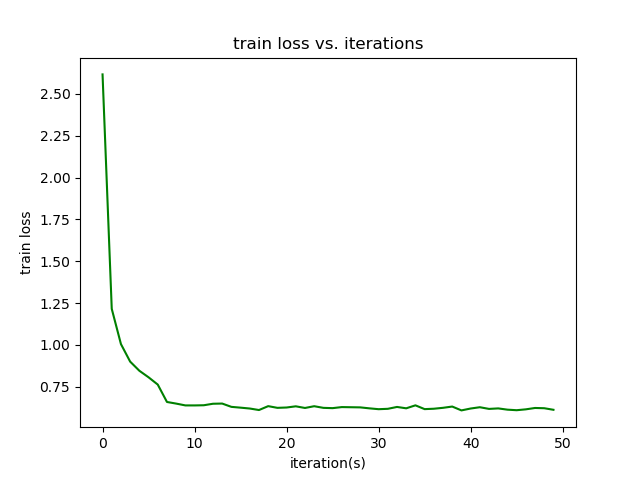
\includegraphics[width=\textwidth]{../results/trainloss_den_adam1}
	\end{minipage}
	\begin{minipage}[t]{0.48\textwidth}
		\centering
		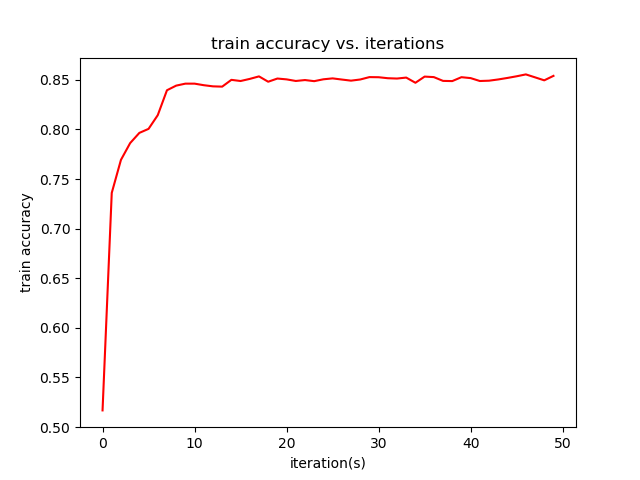
\includegraphics[width=\textwidth]{../results/trainacc_den_adam1}
	\end{minipage}
	\caption{\label{trainres_den_adam1}train loss curve and train accuracy curve using DenseNet121+Adam (with finetuning)}
\end{figure}

\begin{figure}[!h]
	\centering
	\begin{minipage}[t]{0.48\textwidth}
		\centering
		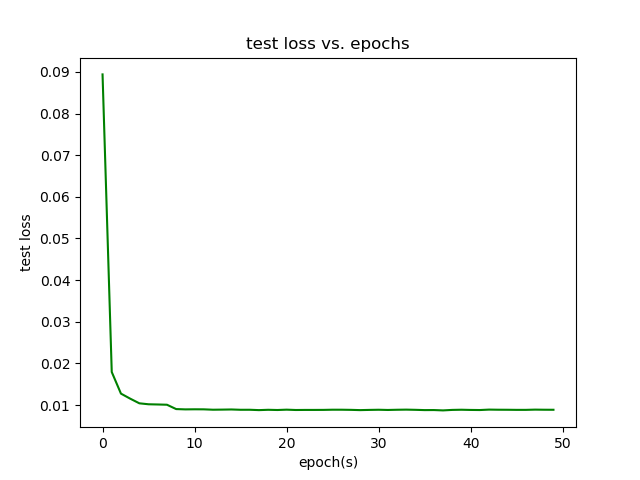
\includegraphics[width=\textwidth]{../results/testloss_den_adam1}
	\end{minipage}
	\begin{minipage}[t]{0.48\textwidth}
		\centering
		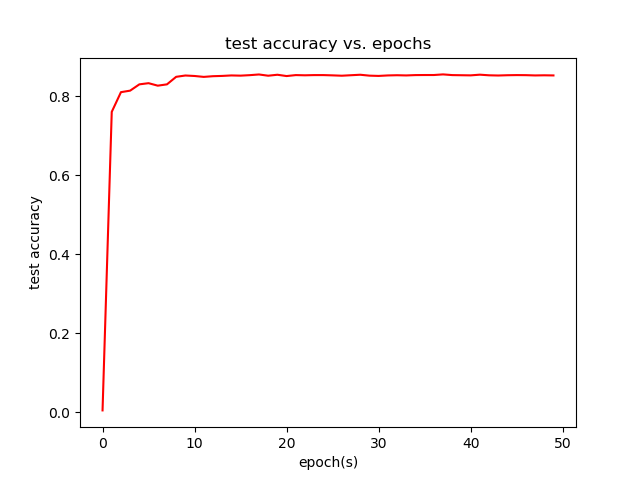
\includegraphics[width=\textwidth]{../results/testacc_den_adam1}
	\end{minipage}
	\caption{\label{testres_den_adam1}test loss curve and test accuracy curve using DenseNet121+Adam (with finetuning)}
\end{figure}

\begin{figure}[!h]
	\centering
	\begin{minipage}[t]{0.48\textwidth}
		\centering
		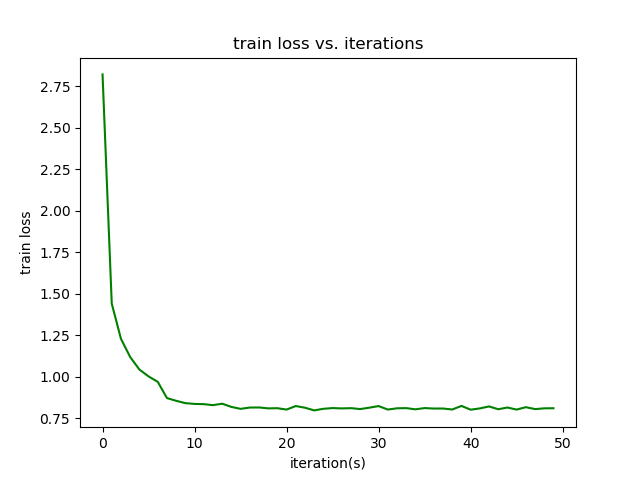
\includegraphics[width=\textwidth]{../results/trainloss_res_adam}
	\end{minipage}
	\begin{minipage}[t]{0.48\textwidth}
		\centering
		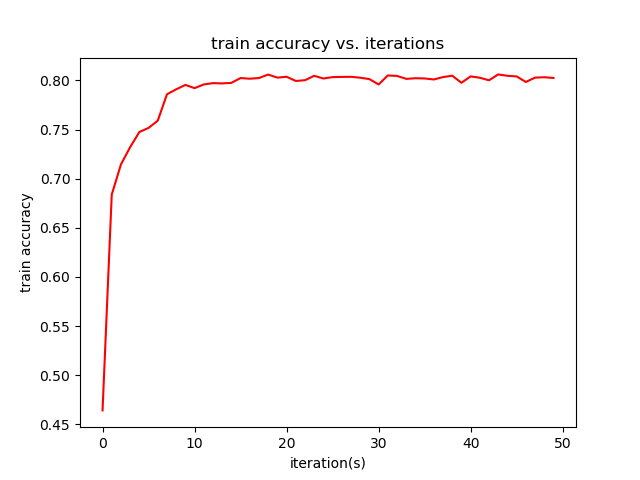
\includegraphics[width=\textwidth]{../results/trainacc_res_adam}
	\end{minipage}
	\caption{\label{trainres_res_adam}train loss curve and train accuracy curve using ResNet18+Adam}
\end{figure}

\begin{figure}[!h]
	\centering
	\begin{minipage}[t]{0.48\textwidth}
		\centering
		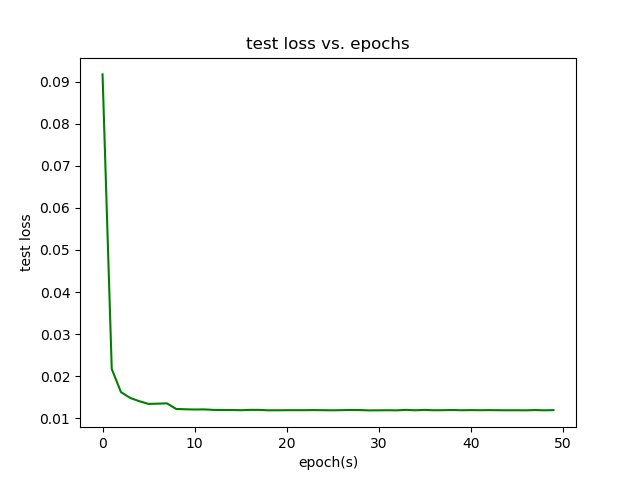
\includegraphics[width=\textwidth]{../results/testloss_res_adam}
	\end{minipage}
	\begin{minipage}[t]{0.48\textwidth}
		\centering
		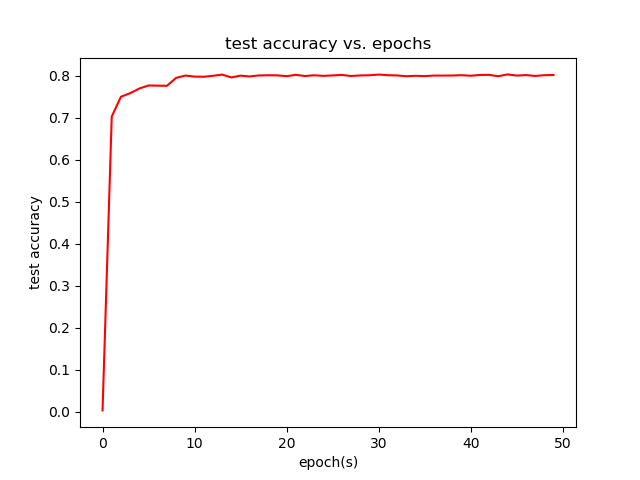
\includegraphics[width=\textwidth]{../results/testacc_res_adam}
	\end{minipage}
	\caption{\label{testres_res_adam}test loss curve and test accuracy curve using ResNet18+Adam}
\end{figure}

\begin{figure}[!h]
	\centering
	\begin{minipage}[t]{0.48\textwidth}
		\centering
		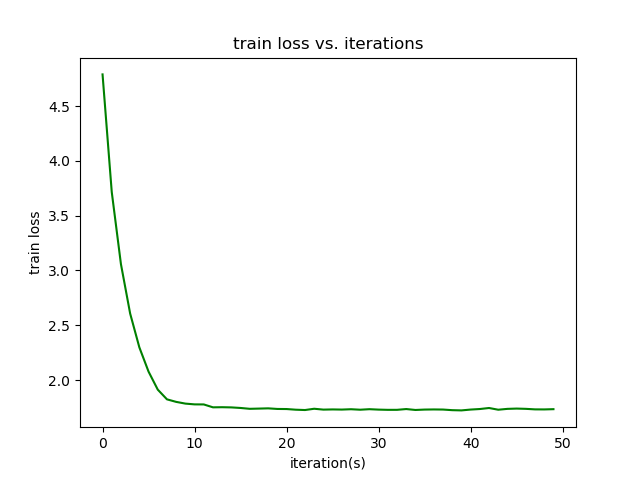
\includegraphics[width=\textwidth]{../results/trainloss_res_sgd}
	\end{minipage}
	\begin{minipage}[t]{0.48\textwidth}
		\centering
		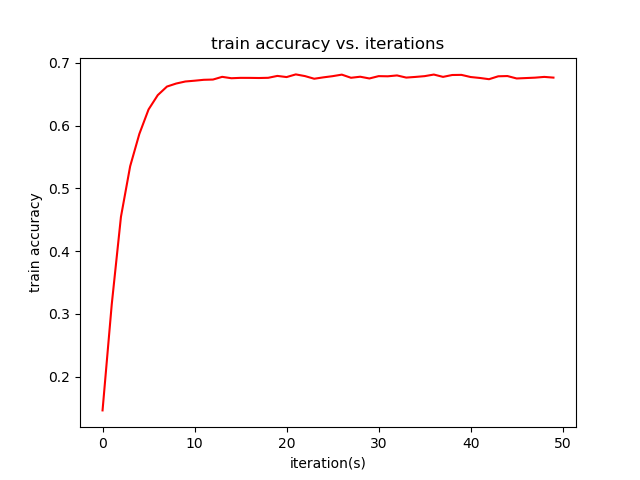
\includegraphics[width=\textwidth]{../results/trainacc_res_sgd}
	\end{minipage}
	\caption{\label{trainres_res_sgd}train loss curve and train accuracy curve using ResNet18+SGD}
\end{figure}

\begin{figure}[!h]
	\centering
	\begin{minipage}[t]{0.48\textwidth}
		\centering
		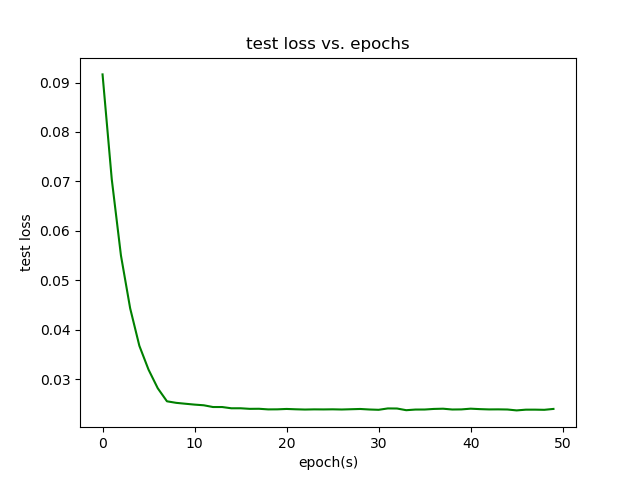
\includegraphics[width=\textwidth]{../results/testloss_res_sgd}
	\end{minipage}
	\begin{minipage}[t]{0.48\textwidth}
		\centering
		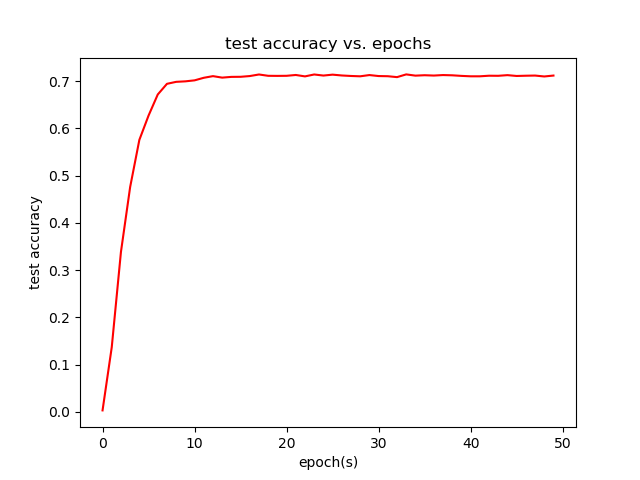
\includegraphics[width=\textwidth]{../results/testacc_res_sgd}
	\end{minipage}
	\caption{\label{testres_res_sgd}test loss curve and test accuracy curve using ResNet18+SGD}
\end{figure}
\chapter{总结与代码说明}
\section{总结}
在本次实验中,我们采用了PCA算法降维、HOG算法提取图像特征、KNN分类、SVM分类、神经网络CNN分类等方式对Caltech 256数据集上的数据进行分类,从分类结果来看,使用神经网络进行分类比使用传统机器学习的方法进行分类的正确率高出很多,这也是为什么最近深度学习很火的原因之一吧,通过神经网络可以提取到一些传统方法提取不到的特征,这样更适合分类,对于神经网络来说,网络结构的定义、损失函数的定义以及参数更新方法都会对最后结果带来一定的影响,本次大作业中使用了ResNet18和DenseNet121等网络结构、交叉熵损失函数、随机梯度下降法和Adam等参数更新方法对此数据集进行分类,从结果对比之中发现DenseNet121网络结构以及SGD参数更新方法在此问题的表现上较优,但是针对不同的问题不同的网络结构会有不同的优势,这需要我们在针对不同问题时多进行尝试找到最优结构,并且我们还可以对数据集进行分析,提出一些创新型的网络结构,或许会有更好的效果。相比较而言,传统方法虽然正确率较低,但是有完整的理论支持,不像神经网络一样是黑盒模型,并且传统模型训练时间也比神经网络方法少很多。

总体来说,本次大作业不仅复习了模式识别课上讲过的一些内容,而且亲自动手实现了相应的算法,并且使用PyTorch对深度学习的算法也进行了一些尝试,学到了很多东西。

\section{代码说明}
本次大作业代码全部使用python3.7完成,文件说明如下:
\begin{itemize}
	\item code\_base文件夹:此文件夹下放置的为基本问题的代码:
	\begin{itemize}
		\item pca\_classify.py:使用PCA+KNN分类的代码;
		\item hog\_svm.py:使用HoG提取特征,SVM分类的代码,其中包含使用PCA降维特征的代码;
		\item create\_train\_neg.py:创建背景类的训练集,此训练集中的图片与所给的test\_neg.txt中均不同;
		\item pca\_classify\_open.py:使用PCA+KNN开集测试分类的代码;
		\item hog\_svm.py:使用HoG提取特征,SVM分类的开集测试代码,其中包含使用PCA降维特征的代码;
	\end{itemize}
	\item code\_additional文件夹:此文件夹下放置的为选做问题的代码:
	\begin{itemize}
		\item create\_train\_test.py:创建选做题部分的训练集和测试集txt文件,并且将文件保存在data\_additional文件夹下
		\item my\_dataset.py:创建适用于pytorch读取图片的Dataset类;
		\item run\_cnn.py:使用CNN进行训练和测试的代码;
		\item pca\_knn.py:使用PCA+KNN在全体数据集上分类的代码;
		\item hog\_svm.py:使用HoG+SVM在全体数据集上分类的代码;
	\end{itemize}
	\item data文件夹:此文件夹下放置的为基础问题所用到的训练集和测试集的txt文件
	\item data\_additional文件夹:此文件夹下放置的为选做问题训练集和测试集的txt文件
\end{itemize}

\chapter{致谢}
\begin{itemize}
	\item 感谢老师一学期以来的辛勤讲述,在课堂上对模式识别的相关算法有了初步的了解,并且从老师分享的自己实验组课题项目中可以学到一些模式识别实战性的经验;
	\item 感谢助教一学期的认真批改作业,辛苦助教了;
\end{itemize}
\end{document}